% Speeding up MDS
% David Lawrence Miller
% d.l.miller@bath.ac.uk
  
\documentclass[a4paper,10pt]{article}
\setlength{\textheight}{22.5cm}
\setlength{\textwidth}{6.47in}
\setlength{\oddsidemargin}{-1mm}
\setlength{\topmargin}{0.1cm}
\setlength{\evensidemargin}{-5mm} 
 
% Load some packages
\usepackage{times, amsmath, amssymb, amsfonts, url, natbib, bm, rotating}
 
\usepackage{multirow}
\usepackage{graphicx}
\usepackage{rotating}

% top matter
\title{Improvements to the MDS+TPRS approach}
\author{David Lawrence Miller\\Mathematical Sciences\\University of Bath\\\texttt{d.l.miller@bath.ac.uk}}
 
% Shortcuts
% Probability
\newcommand{\prob}[1]{\mathbb{P}\left[ #1 \right]}
% Schwarz-Christoffel
\newcommand{\sch}{Schwarz-Christoffel }
% fprime
\newcommand{\fprime}{f^\prime(z)}
% figure reference command
\newcommand{\fig}[1]{\emph{fig.} \ref{#1}}
% Figure reference command
\newcommand{\Fig}[1]{\emph{Fig.} \ref{#1}}
% table reference command
\newcommand{\tabref}[1]{\emph{table} \ref{#1}}
% Table reference command
\newcommand{\Tabref}[1]{\emph{Table} \ref{#1}}
% equation reference command
\newcommand{\eqn}[1]{(\ref{#1})}
% phi inverse
\newcommand{\phiinv}{\phi^{-1}}
% use other phi
\renewcommand{\phi}{\varphi}
%transpose
\newcommand{\tr}[1]{#1^{\text{T}}}
% diagonal
\newcommand{\diag}{\text{diag}}
% call \times \cross
\newcommand{\cross}{\times}

% LaTeX laziness!
\newcommand{\bc}{\begin{center}}
\newcommand{\ec}{\end{center}}
\newcommand{\bn}{\begin{enumerate}}
\newcommand{\en}{\end{enumerate}}
\newcommand{\bi}{\begin{itemize}}
\newcommand{\ei}{\end{itemize}}
\newcommand{\be}{\begin{eqnarray}}
\newcommand{\ee}{\end{eqnarray}}
\newcommand{\bes}{\begin{eqnarray*}}
\newcommand{\ees}{\end{eqnarray*}}
\newcommand{\expect}[1]{\mathbb{E}\left[ #1 \right]}
\newcommand{\tprs}{thin plate regression spline }


\begin{document}
 
% The abstract
%\begin{abstract}
%Here.
%\end{abstract}
 
 
% New theorem for theorems
\newtheorem{thm}{Theorem}[section]
 
%New theorem for definitions
\newtheorem{defn}{Definition}[section]
 
\maketitle

\section{Introduction}

Following from the conclusions of the 12 month report, the main aims from here should be to speed up the algorithm for calculating the within-area distances and improve the accuracy (in terms of mean squared error) of the proposed model. More simulations are also run on different shapes and scenarios to show the stability and generality of using the mDS approach to smoothing. If these objectives are accomplished then the method will be truly competative with the current best approach, soap film smoothing \cite{soap}.


\section{Making the procedure faster}

Previous algorithm slow. Want to speed this up. 

\subsection{Calculating MDS by Lanczos iteration}

The \textsf{R} command used to perform the multidimensional scaling, \texttt{cmdscale}, uses the routine \texttt{eigen} in order to perform the requisite matrix eigendecomposition. This routine will calculate a full eigendecomposition of the matrix, even if only the first $k$ eigenvalues and/or eigenvectors are required. The Lanczos iteration will only calculate the first $k$ eigenvalues (in numeric or algebraic size order.)

The \texttt{igraph} library for \textsf{R} provides an interface to the C++ package \texttt{ARPACK++} which implements the Lanczos procedure. Replacing the \texttt{cmdscale} command with one that uses the \texttt{ARPACK++} interface provided by \texttt{igraph} will decrease the number of computations needed, thus making the calculation of the eigenvalues and vectors faster.

A quick benchmark shows that \texttt{ARPACK++} can compute the first two eigenvalues and vectors faster than just using \texttt{eigen} when the matrix to be eigendecomposed is large. Generating a 1000 by 1000 symmetric matrix of Normal random variates with mean 0 and variance 1000, then performing an eigendecomposition takes 1.68 seconds using \texttt{ARPACK++} and 3.26 seconds using \texttt{eigen} (averaged over 100 runs.) This advantage drops once the matrix is around 100 by 100 and the cost of calling the C++ code begins to dominate; in this case \texttt{ARPACK++} takes 0.037 seconds and \texttt{eigen} takes 0.034 (over 100 runs.) Given that the disadvantage is in the order of hundredths of a second and the advantage is a two-fold decrease in computational time, it makes sense to use the \texttt{ARPACK++} code in all cases.


% sim code is at ~/phd-smoothing/mds/lanczos/time-arpack.R

\subsection{Partial path calculation}

NEED TO THINK ABOUT: do we want to store Euclidean paths? Why? Always more expensive.

Outline: Use sparse grid, calculate paths there, then hook up the new points onto pre-calculated paths there. Hope to get rid of the main part of the calculation (ie. the modifications in the middle where the action hopefully happens.)

Notation is as in algorithm for the path calculation. Taking points $p_i$ and $p_j$ in the set of points in the domain that we wish to find the shortest paths for and drawing a path between them, finding within-area distance with respect to the boundary of $\Gamma$.

This is a modification of the the original algorithm, the routines INIT, DELETE, ALTER, ITER are identical.

\begin{enumerate}
 \item Begin by creating a sparse grid within $\Gamma$ and calculate the non-Euclidean within-area paths between all pairs of points exactly as in algorithm 1. Store these paths as they are calculated as $\mathcal{P}_1,\ldots, \mathcal{P}_M$.
 
\item For each unique pairing of $p_i$ and $p_j$ in the full data set calculate the path use one of the following:

\begin{enumerate}

\item Find a $\mathcal{P}_k$ such that the path between $p_i$ and one end of $\mathcal{P}_k$ and $p_j$ and the other end of $\mathcal{P}_k$ is Euclidean within the $\Gamma$. Join $p_i$ and $p_j$ onto the appropriate ends of $\mathcal{P}_k$ and run ITER until convergence.

\item If there is no Euclidean path between $p_i$ and $p_j$ and any of the ends of $\mathcal{P}_k$, then use the algorithm 1 to calculate the path between $p_i$ and $p_j$. 

\end{enumerate}
\end{enumerate}


\subsubsection{Results}

Comparison to results in previous report to partial path calculation AND Lanczos.


\begin{table}[ht]
\centering
\begin{tabular}{c || c c c c}
 & MDS & Soap film & Thin plate\\ 
\hline
Fit & 3.39225 & 10.87688 & 0.61492\\
Prediction & 4.80357 & 8.87535 & 0.10845\\
\end{tabular}
\label{ramsaytime}
\caption{Average time (in seconds) to fit a realisation of the modified Ramsay horseshoe for the three models considered above. Times are averaged over 100 realisations and were found using the elapsed time provided by \textsf{R}'s built-in \texttt{system.time} function.}
\end{table}

3.6601 
11.77851 
0.56449 
5.34523 
9.55572 
0.1076 




\begin{table}[ht]
\centering
\begin{tabular}{c || c c c c c c}
%  no speedup           speedup
 & MDS & MDS (tensor) & MDS (\textit{pp})& MDS (tensor) (\textit{pp})& Soap film & Thin plate\\ 
\hline
Fit & & & 18.6526 & 19.1409 & 24.6783 & 0.4022\\ 
Prediction & & & 53.5105 & 53.4204 & 29.3946 & 0.1249\\
\end{tabular}
\label{wt2time}
\caption{Average time (in seconds) to fit and predict on a realisation of the peninsula domain for the four models considered above. Times are averaged over 100 realisations and were found using the elapsed time provided by \textsf{R}'s built-in \texttt{system.time} function. For each realisation a sample of size 250 was taken, then a 1253 values were predicted. For the MDS+TPRS models \textit{pp} indicates the cases where the partial paths were pre-calculated, those not marked use algorithm 1.}
\end{table}

% old
%Fit & 84.85242 & 85.35168 & 36.24865 & 0.51721\\
%Prediction & 155.4004 & 155.2419 & 44.22065 & 0.20994 \\




\section{Adjusting the penalty}

Give some intro here.

\cite{wood2000} shows that given some transform of a variable, $y$ say, such that $y_i^\prime=y_i/k$, then $f(x,y^\prime k)$ will give the same fit as $f(x,y)$ (ie. the fit will be the same under the new coordinates) but the penalty will change to:
\begin{equation}
\int\int_\Omega \Big( \frac{\partial^2 f}{\partial x^2} \Big) + 2k\Big( \frac{\partial^2 f}{\partial x \partial y} \Big) + k^3\Big( \frac{\partial^2 f}{\partial y^2} \Big) \text{d}x \text{d}y,
\label{adjustedintegral}
\end{equation}
from the usual penalty:
\begin{equation*}
\int\int_\Omega \Big( \frac{\partial^2 f}{\partial x^2} \Big) + 2\Big( \frac{\partial^2 f}{\partial x \partial y} \Big) + \Big( \frac{\partial^2 f}{\partial y^2} \Big) \text{d}x \text{d}y.
\end{equation*}

This approach will only handle a linear rescaling in one dimension; in the case of the MDS distortions, non-linear rescalings in two dimensions must be addressed. To generalize this concept, a kernel density estimate can be used to vary the penalty over space. Given we have a function of the kernel density estimate, $\mathsf{K}(x,y)$, \eqn{adjustedintegral} can be written as:
\begin{equation}
\int\int \mathsf{K}(x,y) \Big( \Big(\frac{\partial^2 f(x,y)}{\partial x^2}\Big)^2 + 2\Big(\frac{\partial^2 f(x,y)}{\partial y \partial x}\Big) + \Big(\frac{\partial^2 f(x,y)}{\partial y^2}\Big)^2\Big) \text{d}x\text{d}y.
\label{kdeadjust}
\end{equation}



\subsection{Testing in 1 dimension}

Before implementing this approach in full a a test was run in 1 dimension to make sure that this was a feasible adjustment with real benefits. The function:
\be
g(x)=0.2x^{11}(10(1-x))^6+10(10x)^3(1-x)^{10},
\ee
was used and contracted by factors of $20,1,0.05,1$ over the regions $[0,0.4], (0.4,0.6],(0.6,0.8],(0.8,1]$, respectively. The function and it's squashed form are shown in the top panels of \fig{1dadjust}. Evaluating 300, equally spaced, points over the interval $[0,1]$ using a thin plate regression spline and then predicting back onto the same points yielded the blue lines in the lower two plots. The left of these shows the prediction in the transformed space and the right in the original space. The green line was produced using a \tprs with the adjusted penalty matrix elements calculated as follows.

For the moment let us take $f$ to be a one dimensional smooth function. It may be decomposed into its basis function in the usual way:
\be
f(x)=\sum_{\forall j} \beta_j b_j(x) = \tr{\mathbf{\beta}}\mathbf{b}(x).
\ee
In this case, \eqn{kdeadjust} may be written as:
\be
S_{ij}= \int_a^b \frac{1}{\mathsf{K}(x)^3} \frac{\partial^2 b_i(x)}{\partial x^2}\frac{\partial^2 b_j(x)}{\partial x^2} \text{d}x = \int_a^b \frac{1}{\mathsf{K}(x)^3} b^{\prime\prime}_i(x) b^{\prime\prime}_j(x) \text{d}x,
\ee
in one dimension. It is approximated by the midpoint rule as:
\be
S_{ij}= \frac{b-a}{N}\sum_{k=1}^N \frac{1}{\mathsf{K}(x_k)^3} b^{\prime\prime}_i(x_k) b^{\prime\prime}_j(x_k) \quad \text{for} \quad x_k=a+\frac{(k-0.5)(b-a)}{N},
\ee
for $k=1\dots N$. Second derivatives are evaluated by finite differences,
\be
b^{\prime\prime}_i(x) = \frac{ b_i(x+2\epsilon) - 2b_i(x+\epsilon) + b_i(x)}{\epsilon^2}.
\ee

For the sake of efficiency, we infact calculate:
\be
D_{kj}=\sqrt{\frac{1}{\mathsf{K}(x_k)^3}} b^{\prime\prime}_j(x_k),
\ee
for $x_k$ as above. Then $S$ may be calculated as:
\be
S=\frac{b-a}{N}\tr{D}D.
\ee

\begin{figure}
\centering
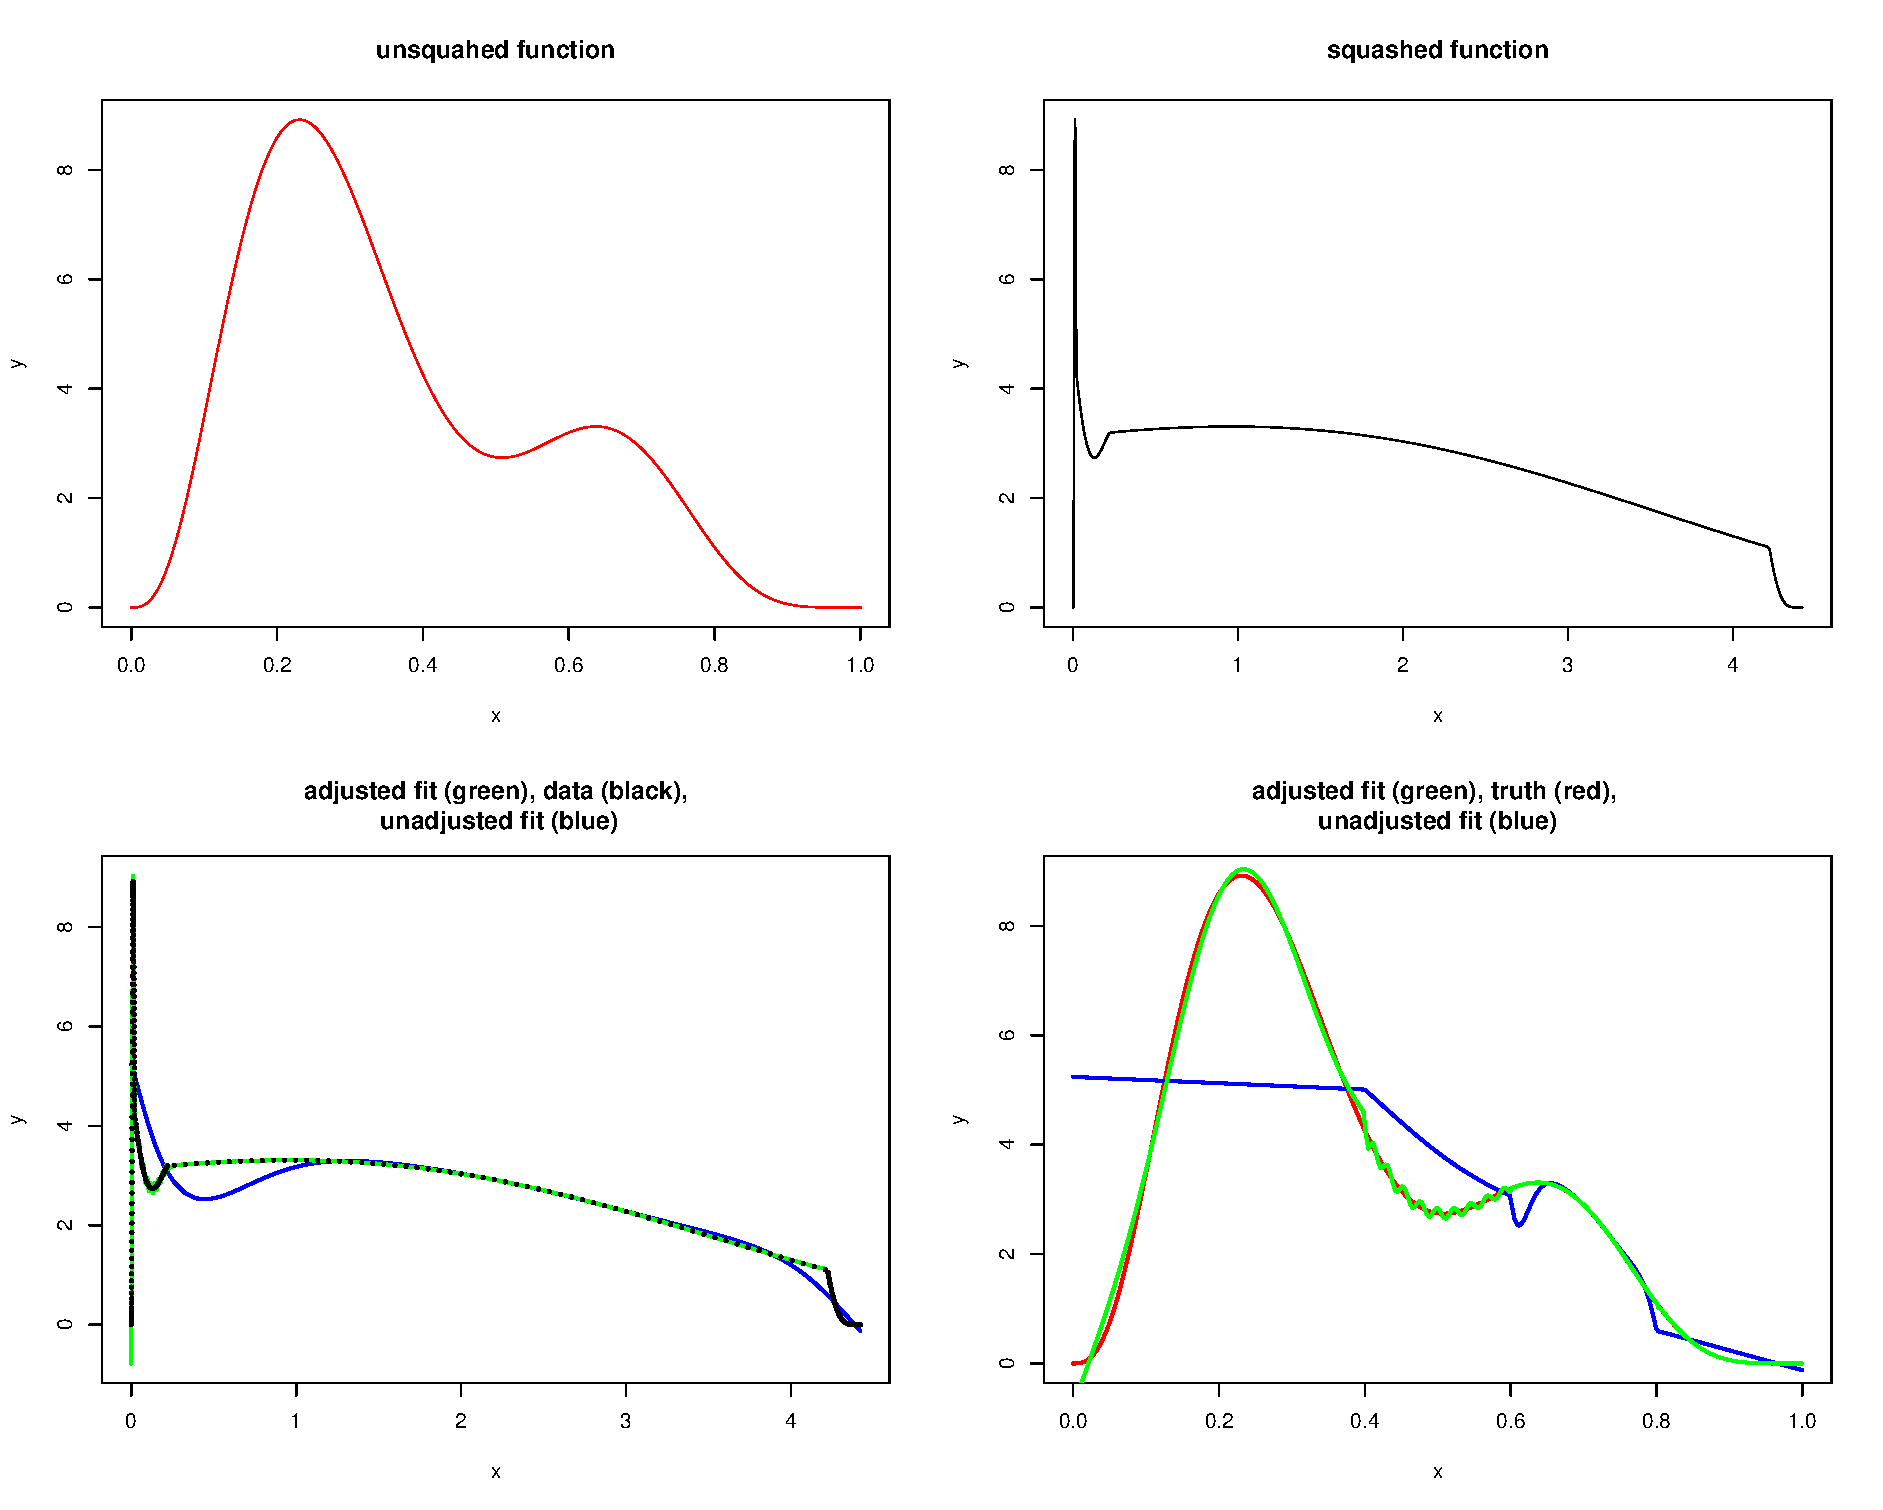
\includegraphics[width=6in]{su-figs/1dadjust.pdf} \\
\caption{}
\label{1dadjust}
% generated by mds/intexp/tpintexp.R
\end{figure}





\begin{table}[ht]
\centering
\begin{tabular}{c c c c c c c c c c}
 & & MSE & &  & EDF & \\ 
 & MDS & MDS (tensor) & soap & thin plate & MDS & MDS (tensor) & soap & thin plate\\ 
0.05  & 0.0354 (0.00033) & 0.0814 (0.01172) & 0.0238 (0.00031) &0.0508 (0.00031) &89.4217 (0.17576) & 87.5388 (0.67077) & 93.8112 (0.85755) & 87.0515 (0.85755)\\ 
0.5  & 0.1015 (0.00082) & 0.0872 (0.00122) & 0.0761 (0.00091) &0.1102 (0.00091) &57.3566 (0.52471) & 45.6116 (0.39864) & 45.1661 (0.69063) & 58.4121 (0.69063)\\ 
5  & 0.9818 (0.03089) & 1.3047 (0.0431) & 1.2253 (0.03584) &1.4379 (0.03584) &7.0495 (0.31291) & 9.6196 (0.39957) & 11.1636 (0.59128) & 12.1361 (0.59128)\\ 
\end{tabular}
\caption{Old results for wt2.}
\end{table}


\begin{table}[ht]
\centering
\begin{tabular}{c c c c c c c}
 & & MSE & &  & EDF & \\ 
 & MDS & soap & thin plate & MDS & soap & thin plate\\ 
0.1  & 0.0033 (3e-05) & 0.0022 (3e-05) & 0.0391 (0.00057) &46.7498 (0.31561) & 38.9315 (0.25237) & 92.6071 (0.08282)\\ 
1  & 0.0426 (0.00104) & 0.0476 (0.00137) & 0.2313 (0.00252) &8.1902 (0.34042) & 10.3035 (0.27974) & 45.9797 (0.3936)\\ 
10  & 2.1158 (0.13359) & 2.5656 (0.15506) & 3.6544 (0.15732) &5.095 (0.28589) & 5.9414 (0.30168) & 7.299 (0.46056)\\ 
\end{tabular}
\caption{Old results for Ramsay}
\end{table}

Some boxplots...

So maybe we just need a less complicated model for the MDS models, this might get rid of some of the extra wigglyness.

Signal to noise ratios $\sigma$=0.05 gives 0.9989871, $\sigma$=0.5 gives 0.9078676, $\sigma$=5 gives 0.09193013 

\begin{figure}
\centering
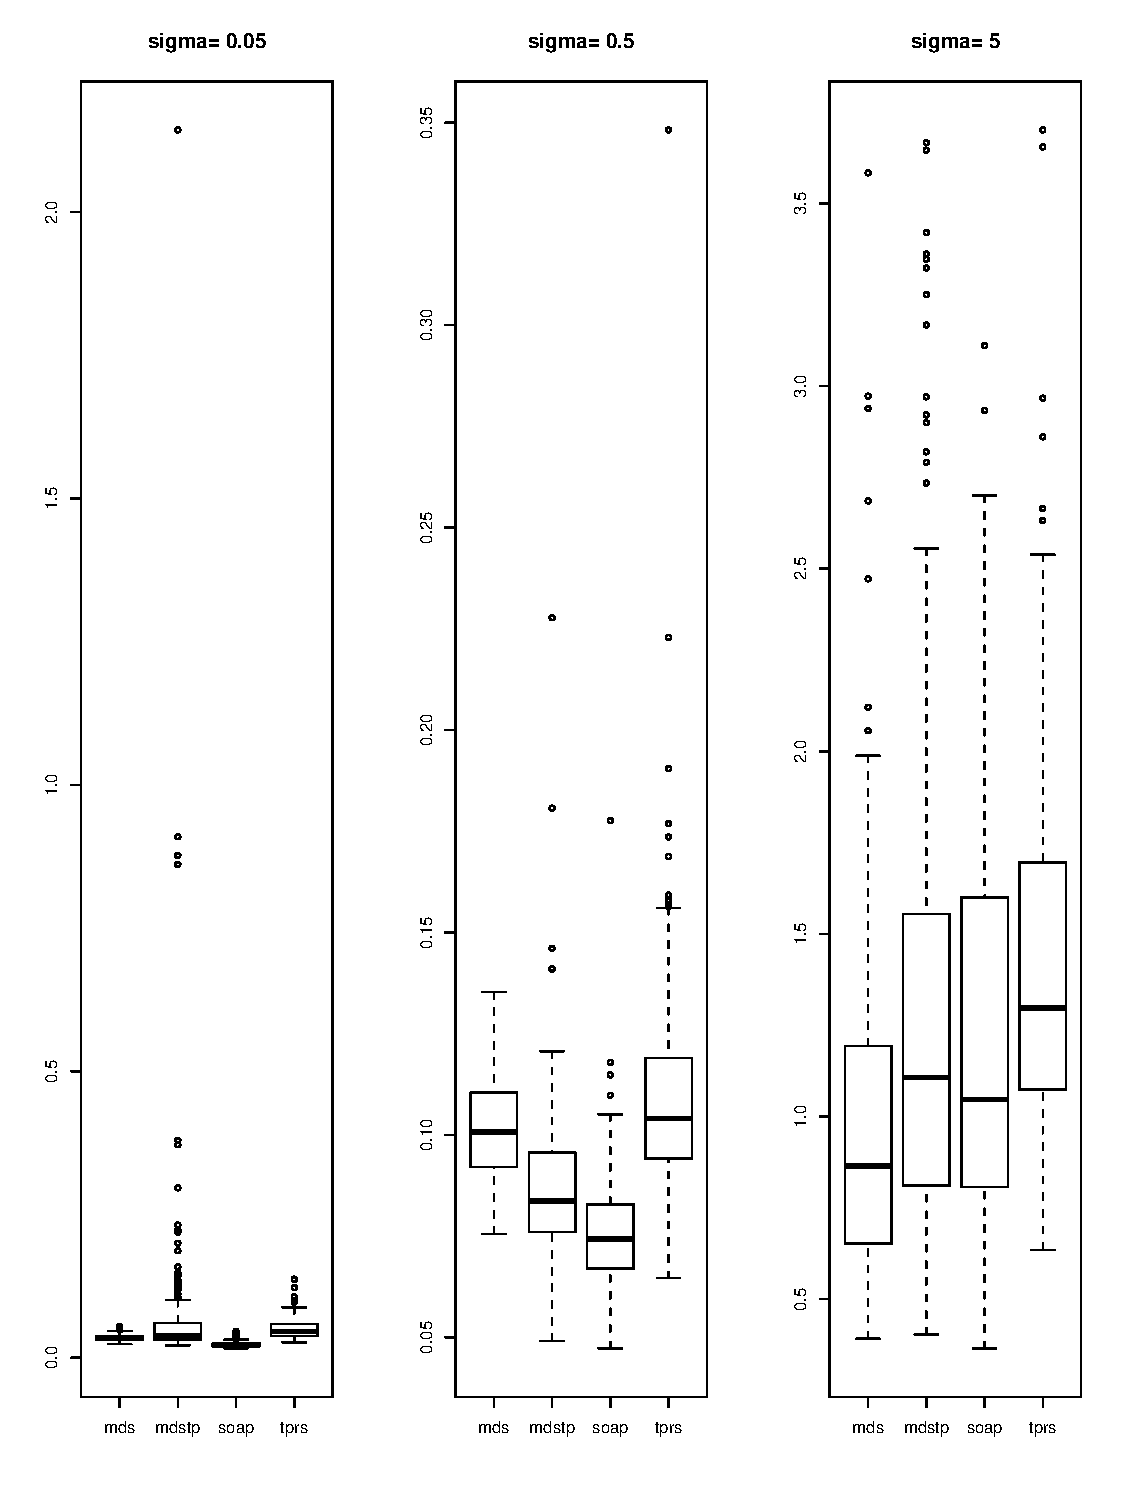
\includegraphics[width=6in]{su-figs/wt2-mds-boxplots.pdf} \\
\caption{MSE performance at various levels of $\sigma$ using no adjustments to penalties for wt2 domain. basis 100}
\label{wt2-boxplots-old}
\end{figure}

\begin{figure}
\centering
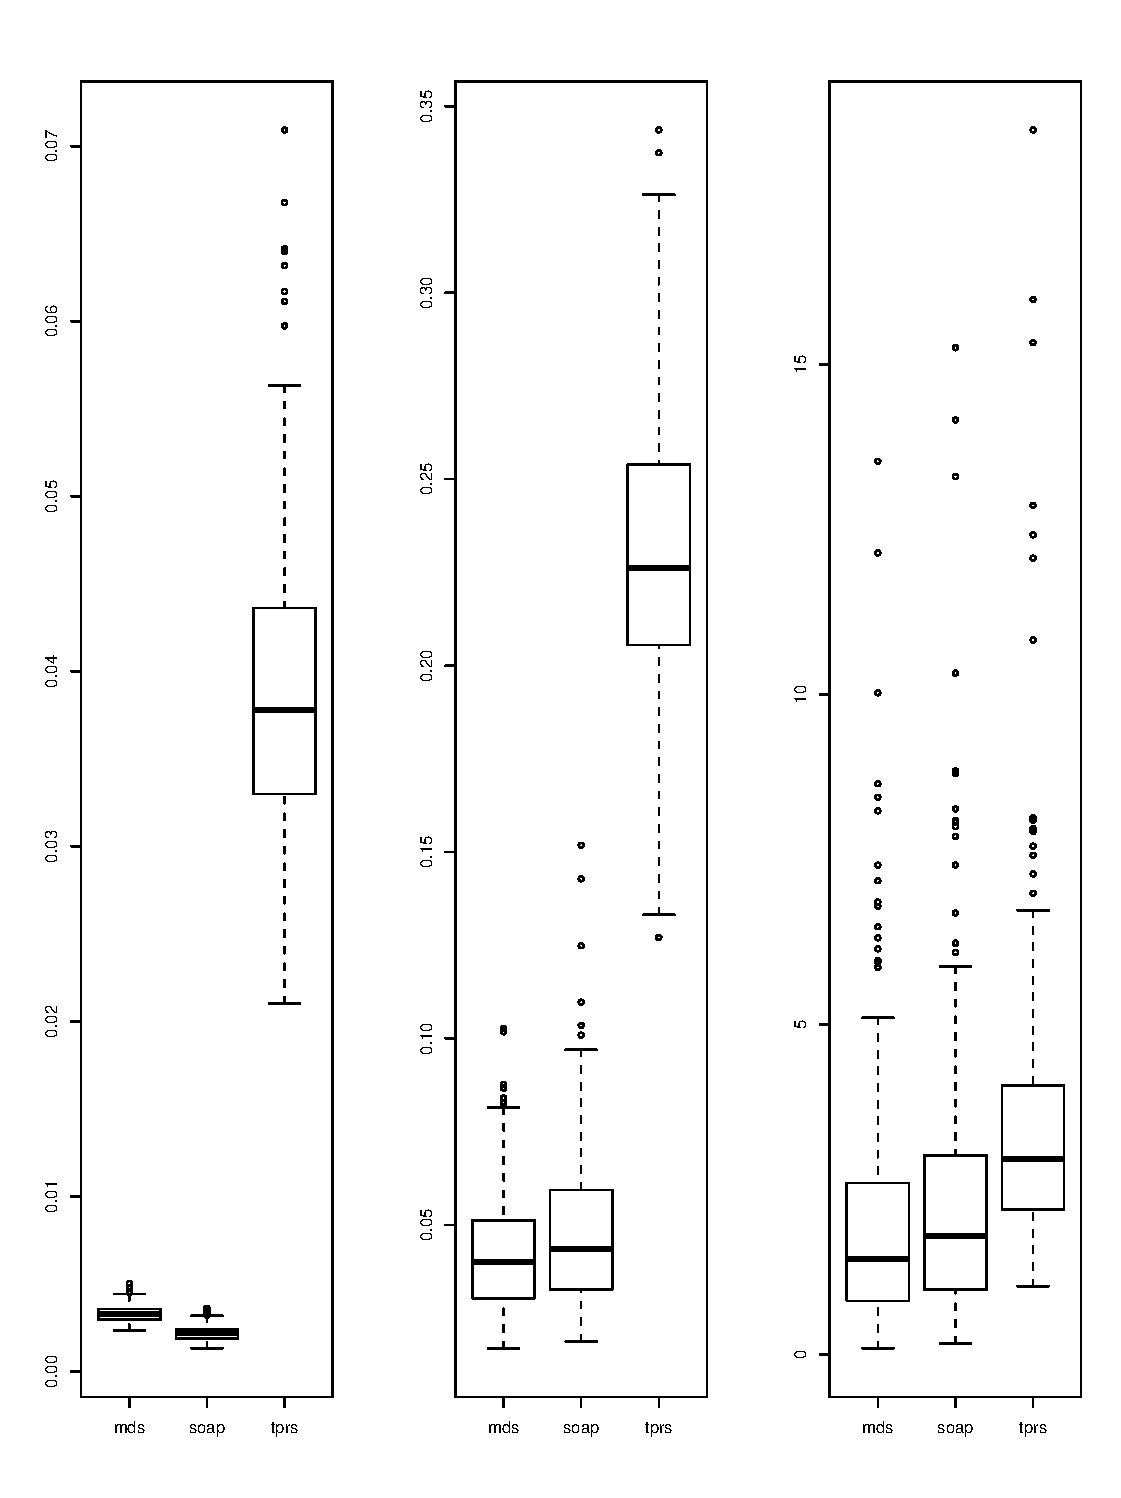
\includegraphics[width=6in]{su-figs/ramsay-mds-boxplots.pdf} \\
\caption{MSE performance at various levels of $\sigma$ using no adjustments to penalties for Ramsay domain.}
\label{ramsay-boxplots-old}
\end{figure}




\subsection{3D?}

\section{Further simulations and analysis}

\subsection{Aral sea}

Good idea to look at real data. Data in soap paper to compare with soap.

Aral sea background. Chlorophil stuff.



\subsection{Spiral}

The shapes investigated so far have been cases where it is rather simple to find the within area paths. We now investigate smoothing over a spiral (idea from \cite{spiralpaper}, courtesy of Vasily Demyanov.) The spiral is defined as:

\begin{equation}
x=\frac{1}{2}\sqrt{\phi}\cos(\phi), \quad y=\frac{1}{2}\sqrt{\phi}\sin(\phi)
\end{equation}



More difficult/esoteric shapes. Take longer to fit, justify using the partial paths

% spiral sample with transformed shape
\begin{figure}
\centering
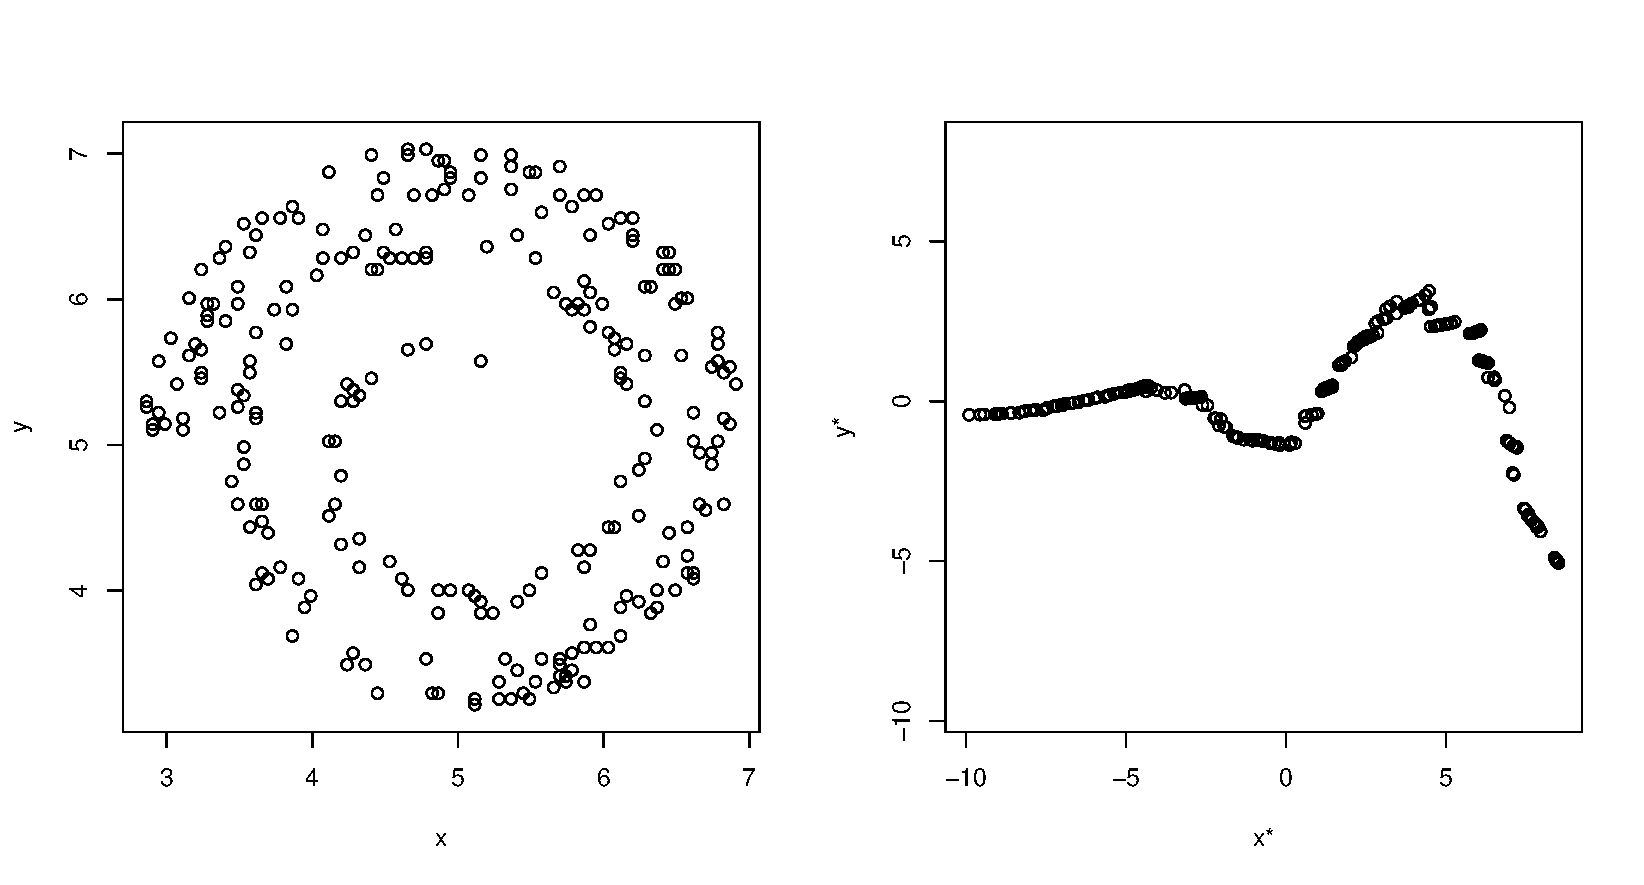
\includegraphics[width=6in]{su-figs/spiralmap.pdf} \\
\caption{A random sample of 250 points from the spiral, and it's mapping in MDS space.}
\label{spiralmap}
% generated spiralmap.R
\end{figure}




\bibliographystyle{plainnat}
\bibliography{mds-refs}

\end{document}
